
\subsection{Oppsett av UWB-tags og ankere}
Det første oppsettet av UWB-tags og ankere ble gjort på et grupperom. Ankerene ble plassert i henhold til Pozyx sin guide. 
Guiden sier at ankerene skal bli plassert:
\begin{itemize}
\item Høyt og i synsrekkevidde for taggen
\item Ikke i en rett linje, men rundt i rommet.
\item 2-20 meter fra hverandre
\item 20 cm vekk fra metall
\item Vertikalt, slik at antennen peker opp eller ned
\item I ulik høyde for å oppnå 3D posisjonering
\item I synsrekkevidde til hverandre dersom man ønsker å bruke auto kalibrering
\end{itemize}


(Pozyx, n.d.)
Ankerene ble plassert i vært hjørnet av rommet slik som figur \ref{fig:ankerplassering} viser. 
Det ene ankeret ble plassert høyere enn de andre for å oppnå 3D posisjonering.
Hjørnet nærmest det ene ankeret (ankeret til høyre på Figur 25) ble brukt som nullpunkt. 
Det ble brukt laser for å måle opp de andre ankrenes posisjon i forhold til dette punktet. 
Gulvet i rommet ble regnet som høyde 0. Ankerenes posisjoner i millimeter ble da:

\begin{center}
\begin{tabular}{||c c c c||} 
 \hline
 Anker ID & x-retning & y-retning & z-retning \\ [0.5ex] 
 \hline\hline
 0x0D7A & 27 & 44 & 1132 \\ 
 \hline
 0x6834 & 27 & 2787 & 2415 \\
 \hline
 0x684E & 4725 & 494 & 1165 \\
 \hline
 0x684F & 4725 & 2795 & 1184 \\ [1ex] 
 \hline
\end{tabular}
\end{center}

\begin{figure}[htp]
\centering
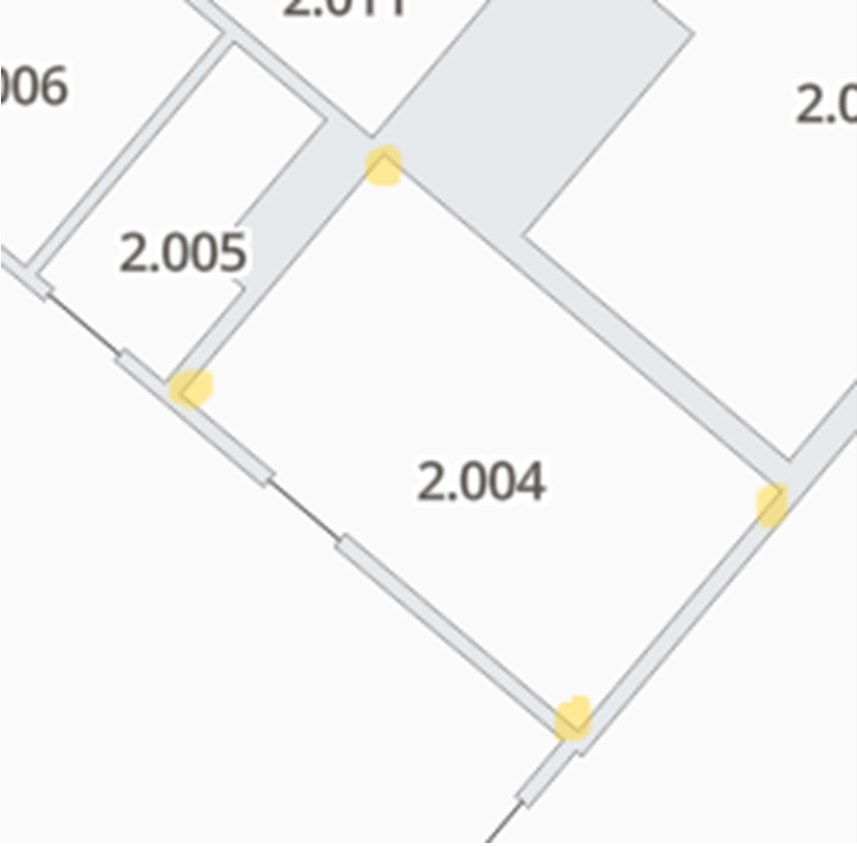
\includegraphics[width=0.5\columnwidth]{figures/ankerplassering}
\caption{Ankerplassering}
\label{fig:ankerplassering}
\end{figure}

Når ankrene var målt opp ble oppmålingen lagt inn i Pozyx Creator Controller, vist i figur \ref{fig:creator-controller}. 
Dette programmet ble brukt til å bekrefte at systemet fungerte, og at tagen greide å finne posisjonen sin.

\begin{figure}[htp]
\centering
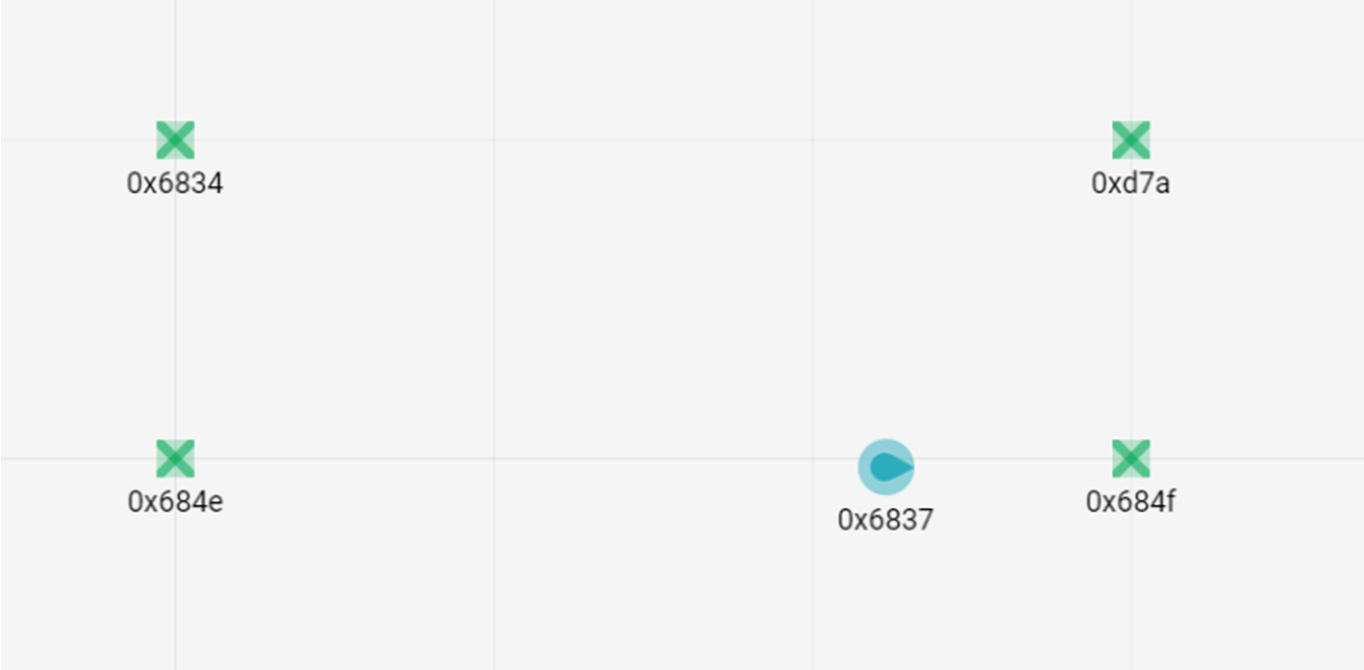
\includegraphics[width=0.5\columnwidth]{figures/creator-controller}
\caption{Pozyx creator controller}
\label{fig:creator-controller}
\end{figure}

\subsection{Avlesning av posisjon med Arduino}
For å kunne bruke dataen fra Pozyx på flightcontrolleren til quadcopteret måtte dataen oversettes til MavLink. 
Til dette ble det brukt en Arduino Nano. Arduinoen ble loddet opp til Pozyx tagen som vist i figur \ref{fig:arduino-tag}.
indoorLoiter (Mackay, 2016), et Arduino program skrevet av Ardupilot, ble brukt på Arduinoen. 
Dette programmet henter data fra Pozyx tagen, oversetter det til MavLink, og sender det deretter ut til Pixhawken.

\begin{figure}[htp]
\centering
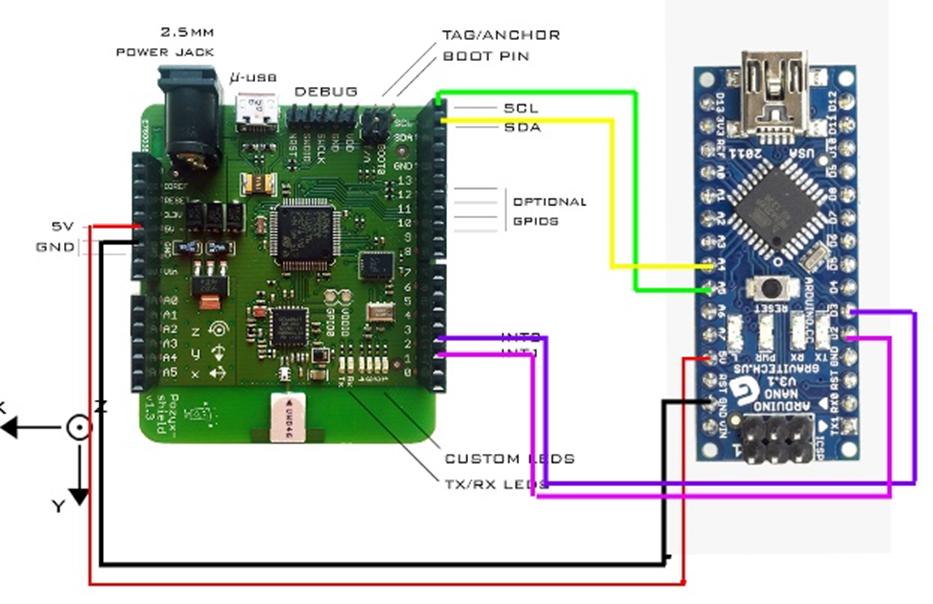
\includegraphics[width=0.5\columnwidth]{figures/oppkobling2}
\caption{Oppkobling av pozyx tag og arduinor}
\label{fig:arduino-tag}
\end{figure}
 
I første omgang ble dette programmet brukt for å teste at Arduinoen faktisk greide å lese av posisjon fra Pozyx tagen, 
og se på nøyaktigheten til systemet.

\subsection{Plotting med python}
Når indoorLoiter programmet kjører på Arduinoen så sender Arduinoen ut posisjonen til tagen i x, y og z retning på USART. 
Dette ble brukt til å lese av posisjonen på en datamaskin som kjørte python, og plotte posisjonen over ulike tidsrom.
Figur \ref{fig:ovenfra} viser et ovenfra plot fra en test der tagen ble beveget rundt i grupperommet. 
Figur \ref{fig:ovenfra} viser et plot fra samme test, men fra siden. 
Plotene viser at posisjonen i x-y retning er mye mer presis enn posisjonen i z retning. 
Det ble ikke gjort mye arbeid for å forbedre dette, da høydeholdet på dronen uansett bruker barometer.

\begin{figure}[htp]
\centering
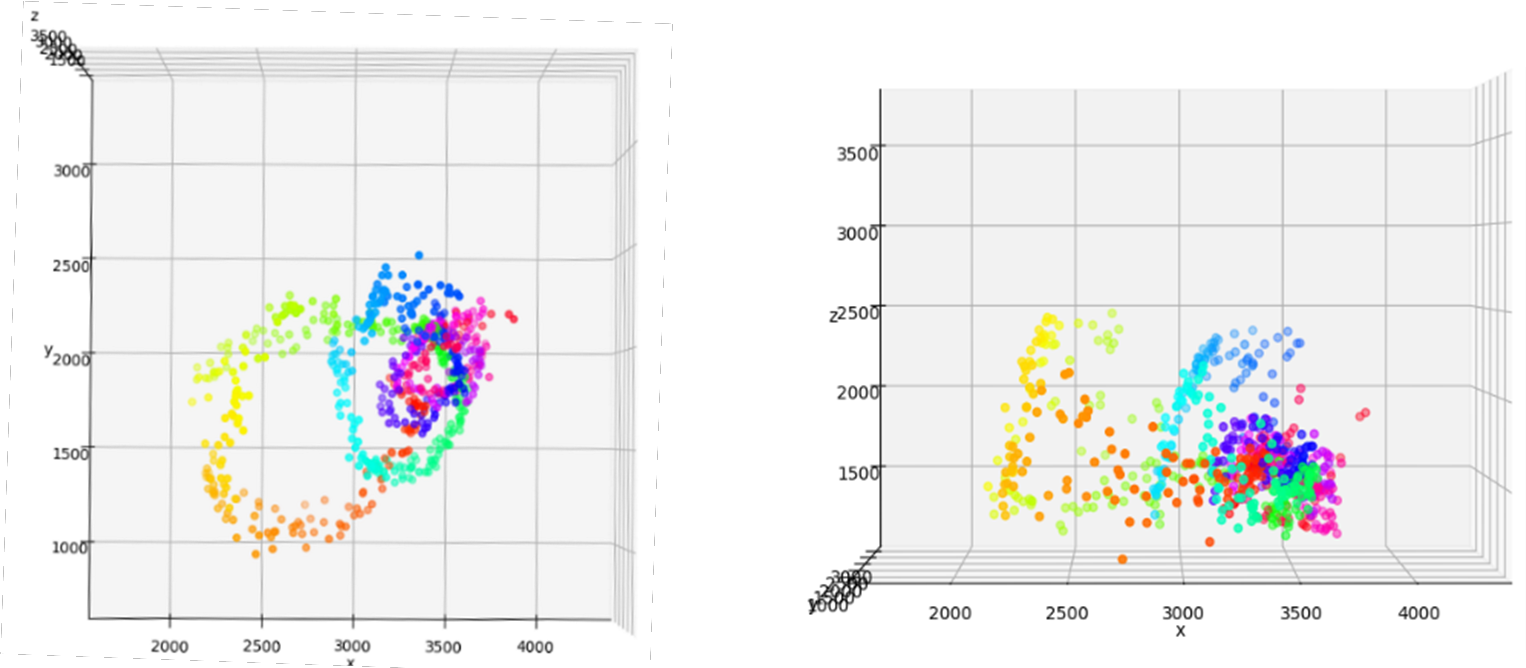
\includegraphics[width=0.5\columnwidth]{figures/plott-ovenfra}
\caption{Plot fra innendørstest. x-y planet i figuren til høyre, x-y planet i figuren til venstre.}
\label{fig:ovenfra}
\end{figure}

\subsection{Presisjon og rekkevidde av UWB system}
Hensikten med denne øvelsen var å teste presisjonen og rekkevidden til UWB systemet. 
Testene ble gjort ute, ved å enten gå rundt med en tag eller la en tag stå festet til en tripod.

\subsubsection{Rekkevidde}
Først ble det utført en test for å se på rekkevidden til systemet. 
RSSI (Received Signal Strength Indicator) ble brukt som en indikator på hvor sterkt signal som ble mottatt, 
og dette ble sammenliknet med avstanden det ble målt over. 
Testen ble gjennomført ved å sette et anker på en tripod, og en tag på en annen tripod. Avstanden mellom disse ble målt opp med målebånd, 
da det var for sterkt lys til å måle opp med laser. De tre første loggingene ble gjennomført på 5 meter, 
og deretter ble tagen flyttet lengre og lengre vekk fra ankeret for vær logging, fem meter om gangen helt opp til 40 meter. 
En logging varte i 20 sekunder, og ga ca. 120 målinger. Figur \ref{fig:RSSI1} viser dataen fra loggene. 
Det øverste plotet viser gjennomsnitts verdien for hver avstand. Det viser en sterk trend på at signalet blir 
svakere når avstanden øker. Plotet under viser at på hver log holder RSSI målingene seg stabilt, med en nøyaktighet på ± 2dBm.

\begin{figure}[htp]
\centering
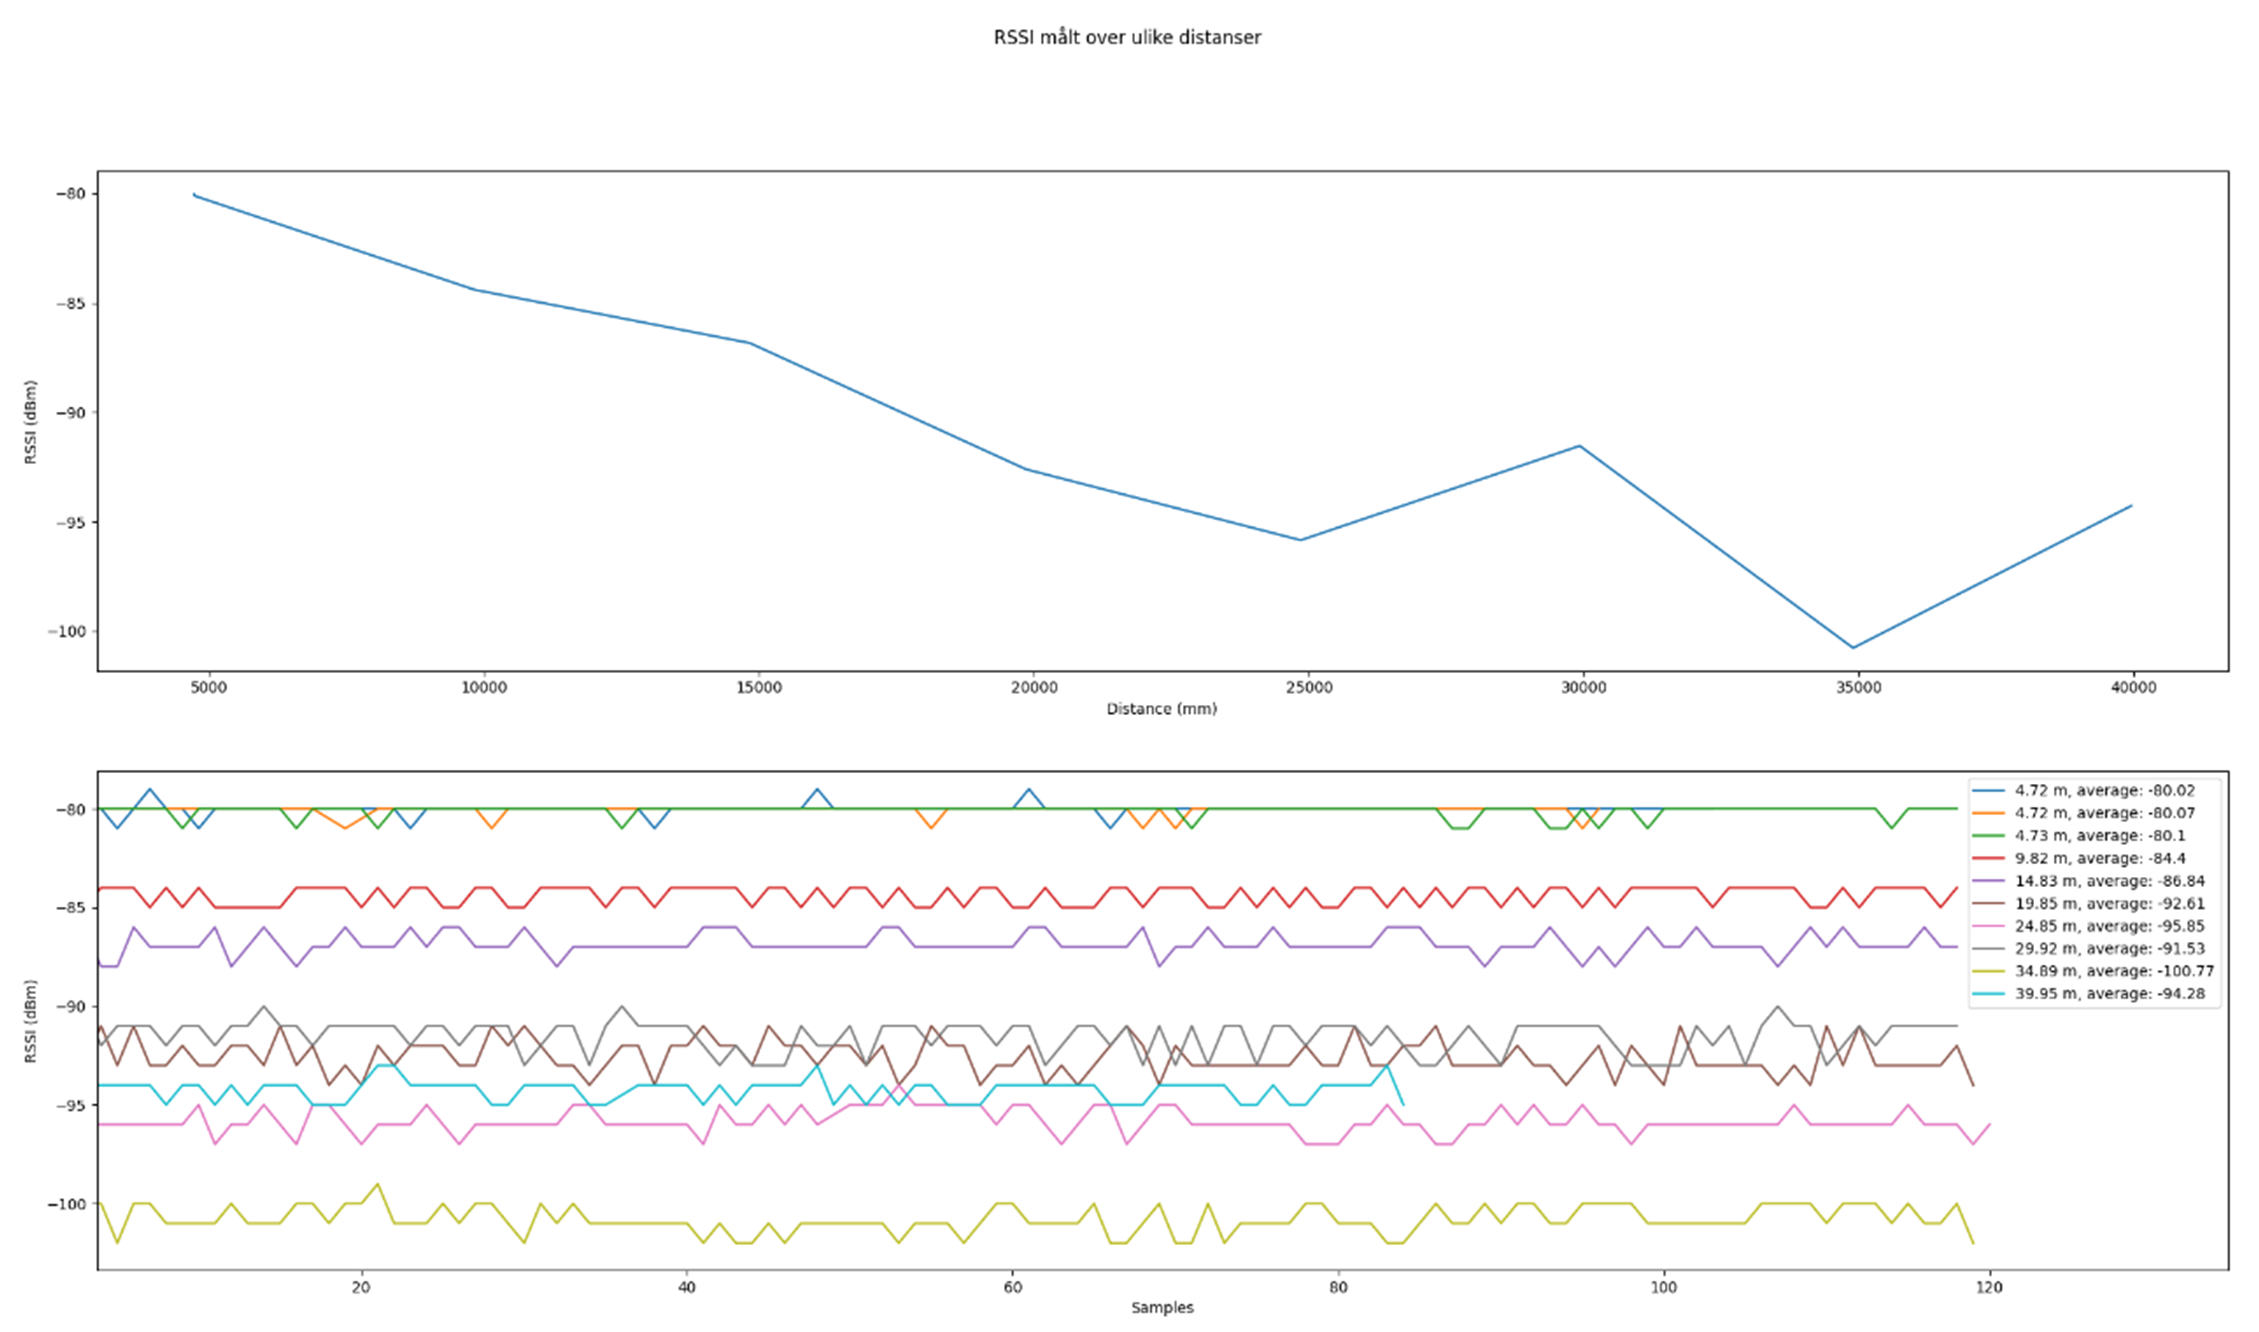
\includegraphics[width=0.5\columnwidth]{figures/rssi-test-ute}
\caption{RSSI måling over ulike distanser.}
\label{fig:RSSI1}
\end{figure}

Det ble også gjennomført en test der tagen ble holdt i hånden, og flyttet fra ca. 5 meter til ca. 80 meter. 
Figur \ref{fig:RSSI2} viser resultatene fra denne testen. Bortsett fra et lite avvik helt i starten av testen, 
så viser dette plotet samme trend som tidligere. RSSI verdiene blir svakere når avstanden øker.

\begin{figure}[htp]
\centering
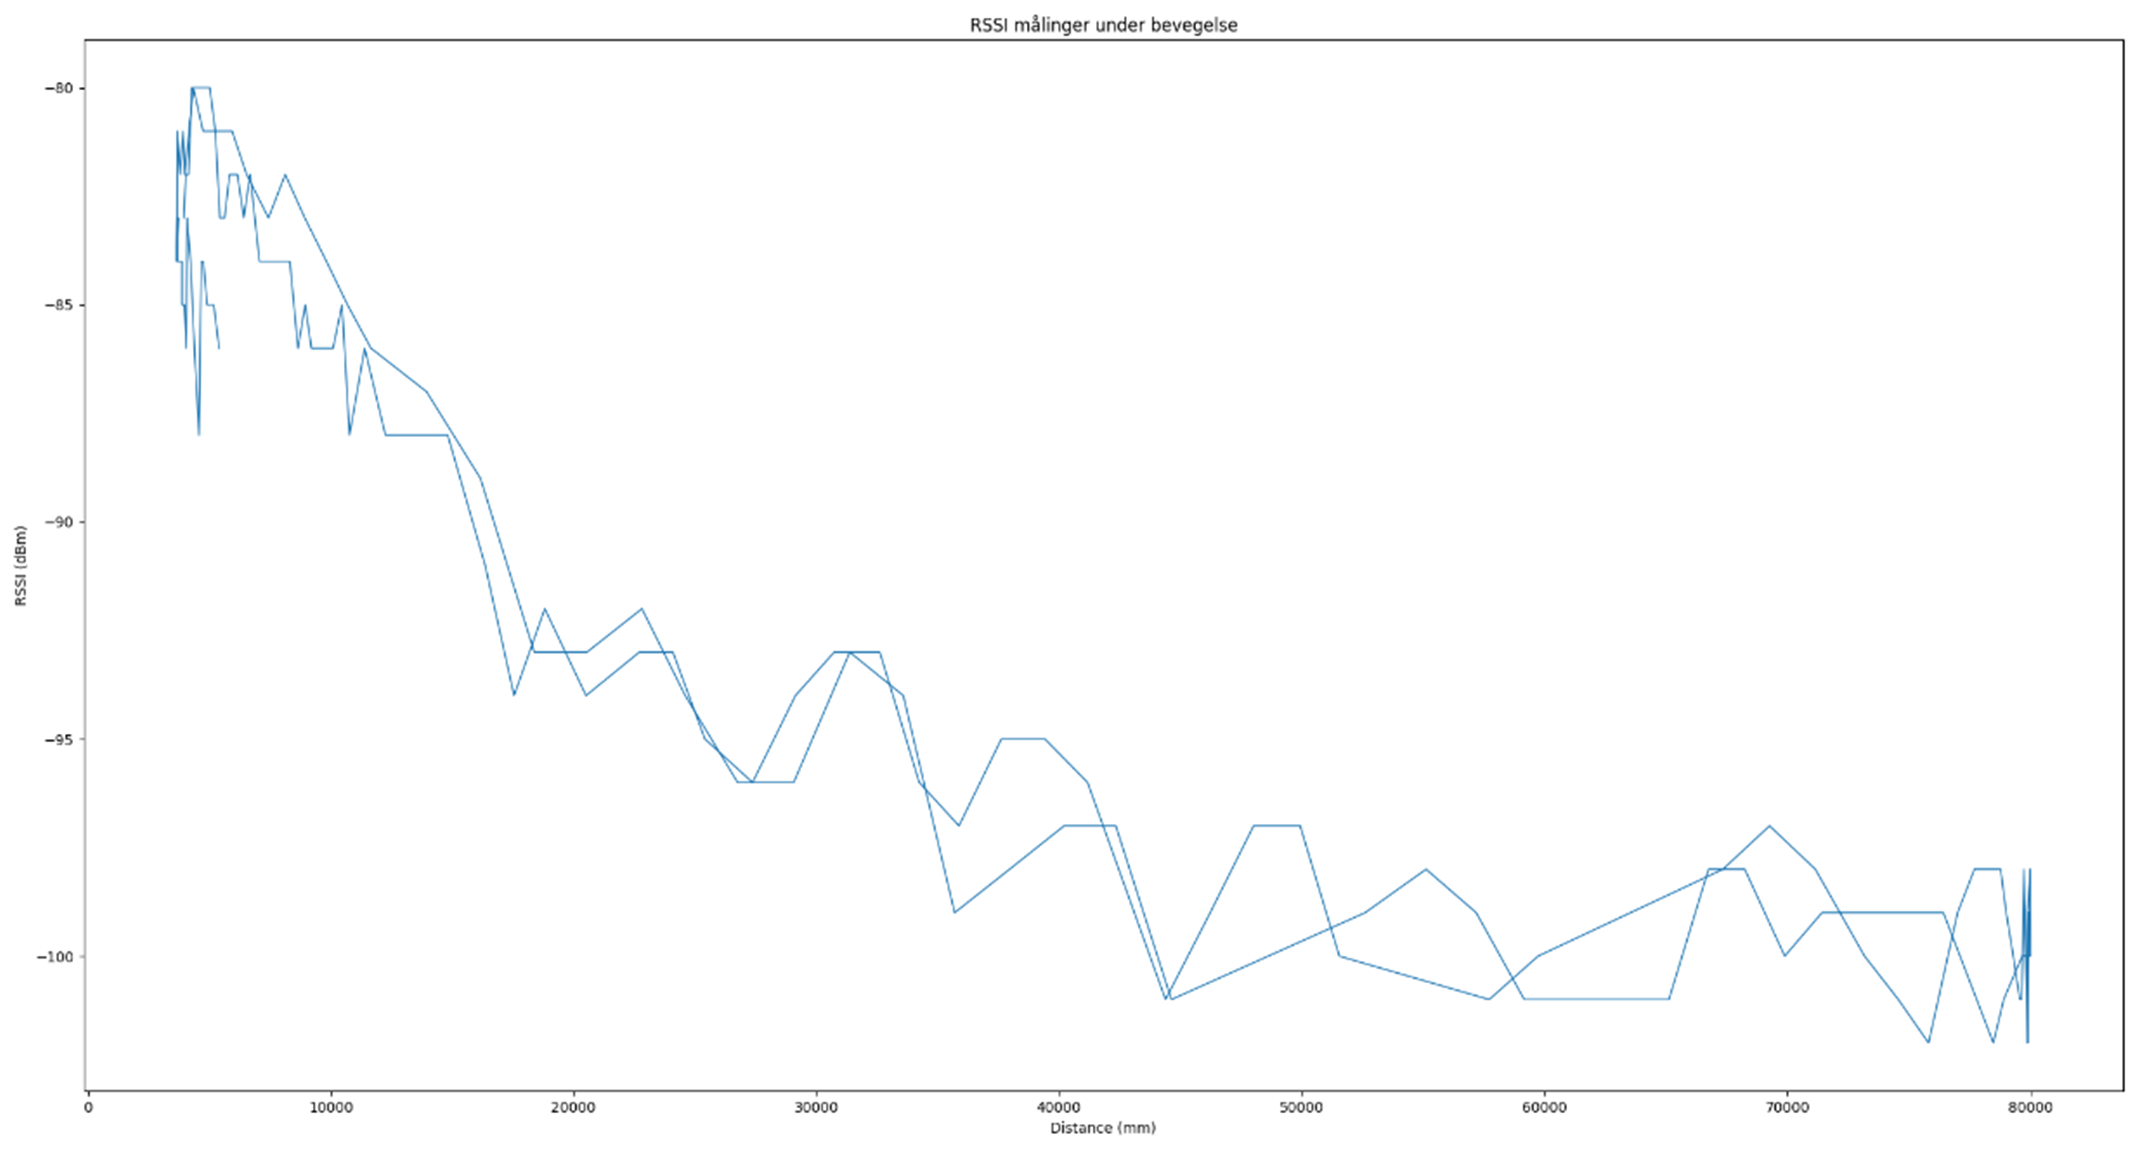
\includegraphics[width=0.5\columnwidth]{figures/rssi-test-ute2}
\caption{RSSI måling over ulike distanser.}
\label{fig:RSSI2}
\end{figure}

\newpage
\subsubsection{Presisjon}
Det ble utført presisjonstester med to ulike anker oppsett. 
De fire første testene ble gjennomført som vist i figur \ref{fig:oppsett}, 
resterende syv tester ble gjennomført slik Figur 15 viser. 
Det ble skrevet et python program for logging av dataen fra Pozyx, 
og et python program for plotting og analyse. 

\begin{figure}[htp]
    \centering
    \subfloat[\centering $2\cdot2 m$]{{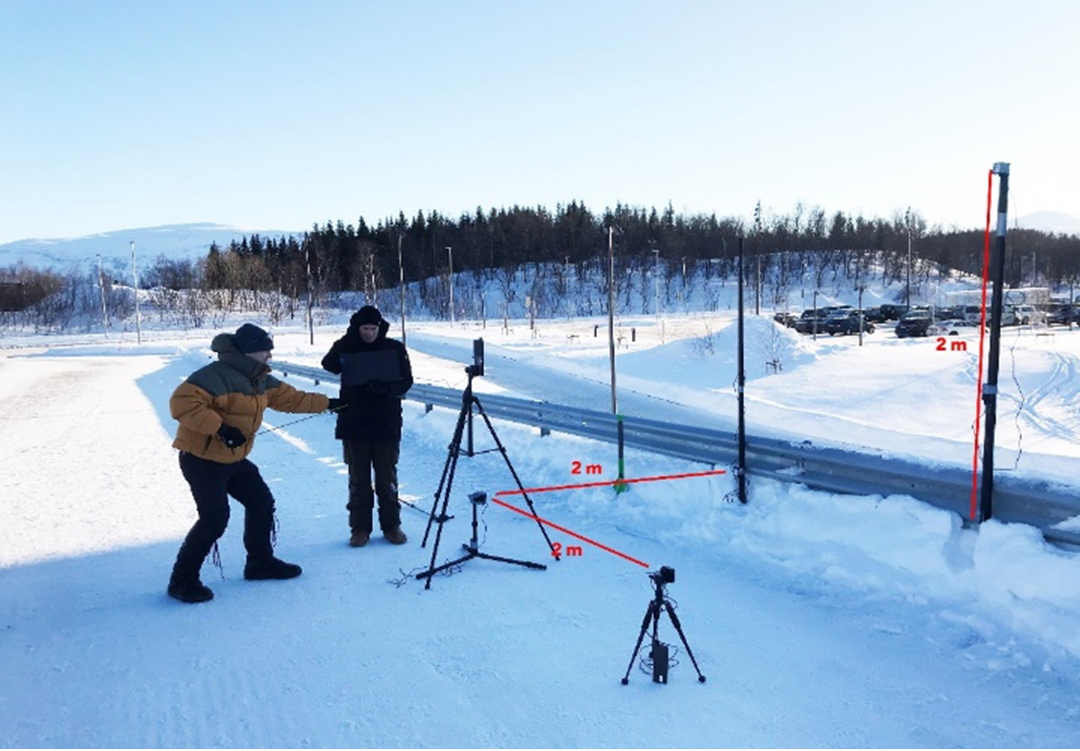
\includegraphics[width=5cm]{figures/ankere2x2} }}%
    \qquad
    \subfloat[\centering $5\cdot5 m$]{{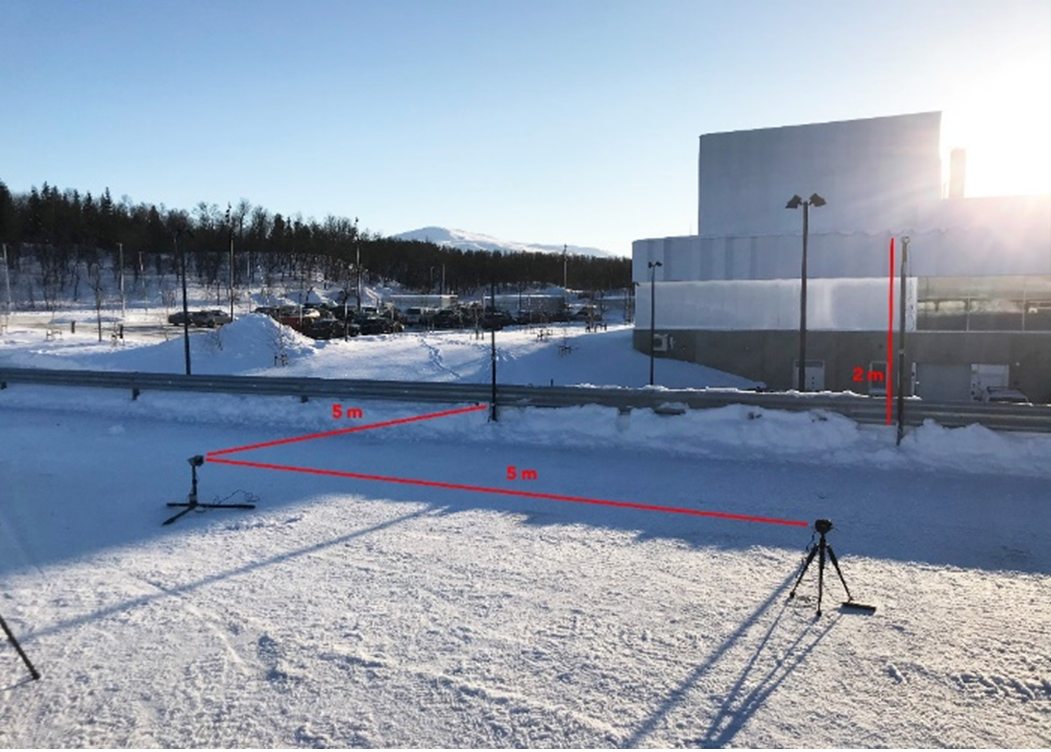
\includegraphics[width=5cm]{figures/ankere5x5} }}%
    \caption{Ulike anker oppsett.}%
    \label{fig:oppsett}%
\end{figure}

Den svarte firkanten i Figur \ref{fig:2x2målinger} og Figur \ref{fig:2x2målinger50} illustrerer 
posisjonen til ankerene i 2x2 meter oppsett, der ankrene er plassert i hvert sitt hjørne. 
Her er målingene plottet etter tid, der det første punktet er lilla og det siste er gult. 

\begin{figure}[htp]
\centering
\includegraphics[width=0.5\columnwidth]{figures/målinger-2x2}
\caption{Målinger med $2\cdot2 m$ ankere.}
\label{fig:2x2målinger}
\end{figure}
\begin{figure}[htp]
\centering
\includegraphics[width=0.5\columnwidth]{figures/målinger-2x2-minus50}
\caption{Målinger med $2\cdot2 m$ ankere uten de 50 første målepunkter.}
\label{fig:2x2målinger50}
\end{figure}

Somf figur \ref{fig:2x2målinger} viser er det mye feilmålinger helt i starten av loggingene. 
I figur \ref{fig:2x2målinger50} er derfor de 50 første målingene fjernet, som omtrent tilsier de første 2 sekundene. 
Tabellene under viser et utdrag fra noen av målingene, med plot og resultater. I utregningene er også de 50 første målingene fjernet.

\begin{figure}[htp]
\centering
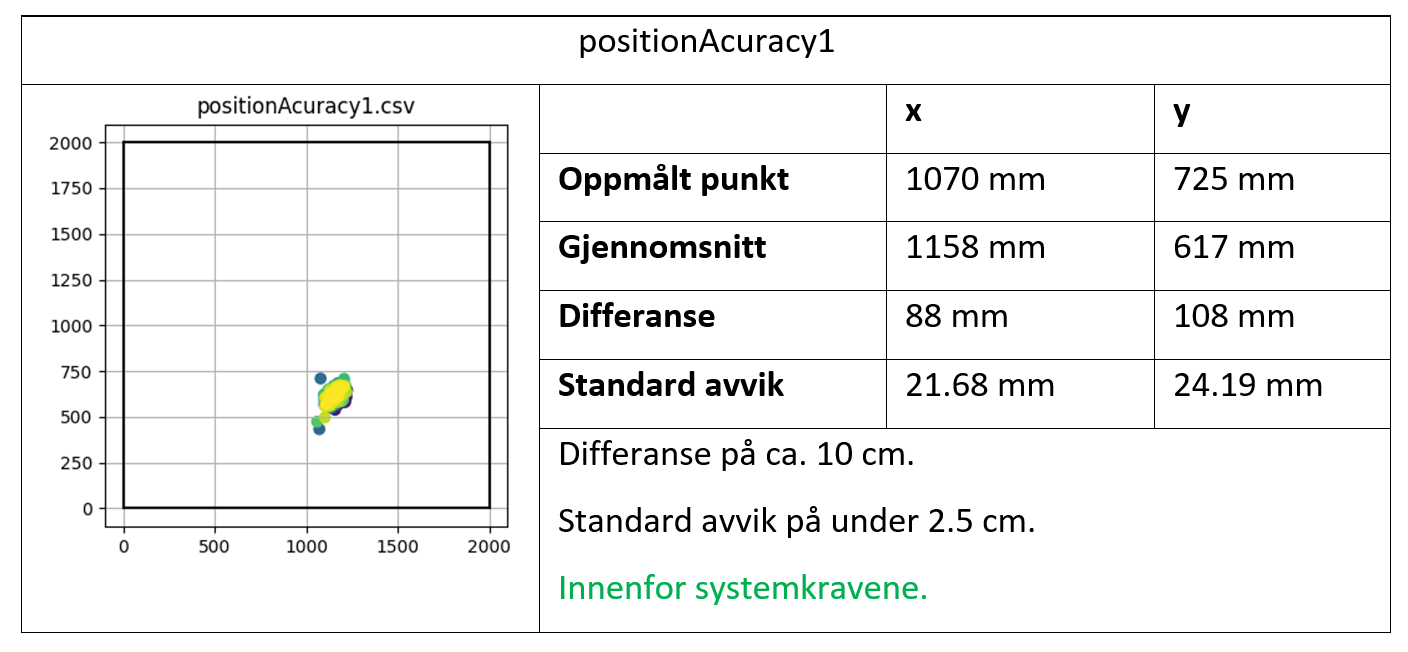
\includegraphics[width=0.5\columnwidth]{figures/2x2resultat1}
\caption{Resultater fra måling 1.}
\label{fig:2x2res1}
\end{figure}
\begin{figure}[htp]
\centering
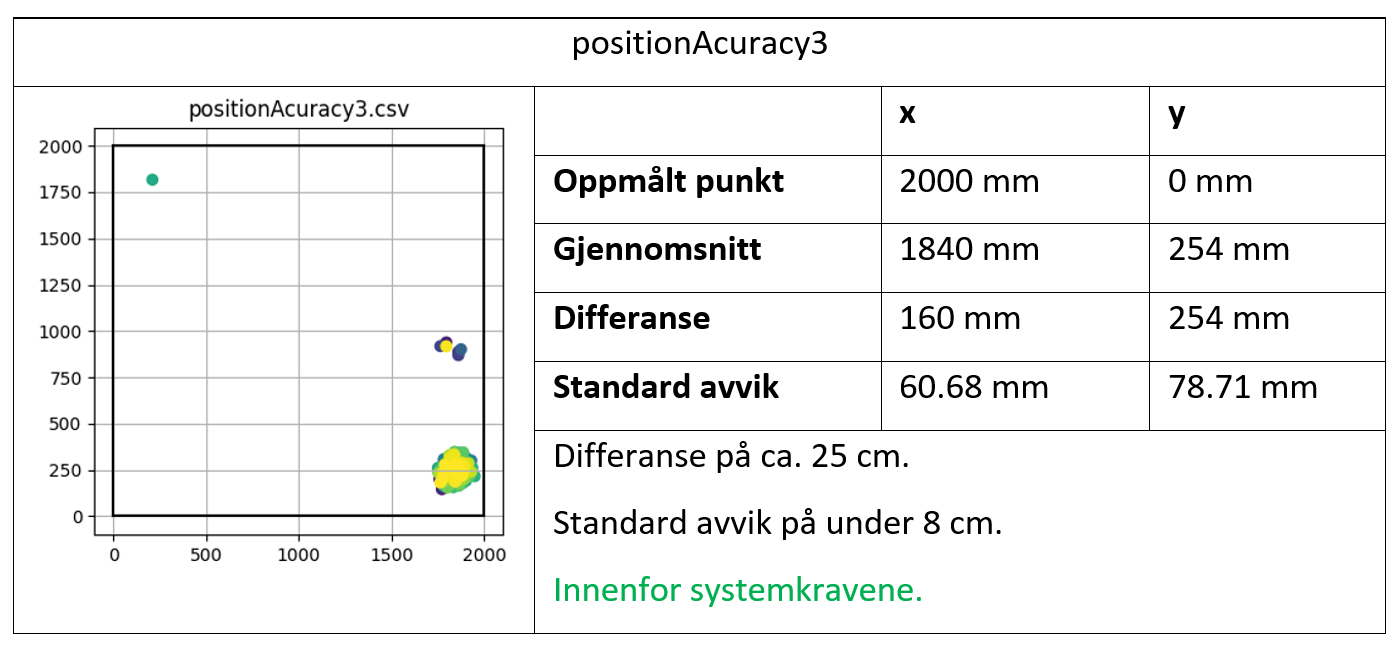
\includegraphics[width=0.5\columnwidth]{figures/2x2resultat3}
\caption{Resultater fra måling 3.}
\label{fig:2x2res3}
\end{figure}
\begin{figure}[htp]
\centering
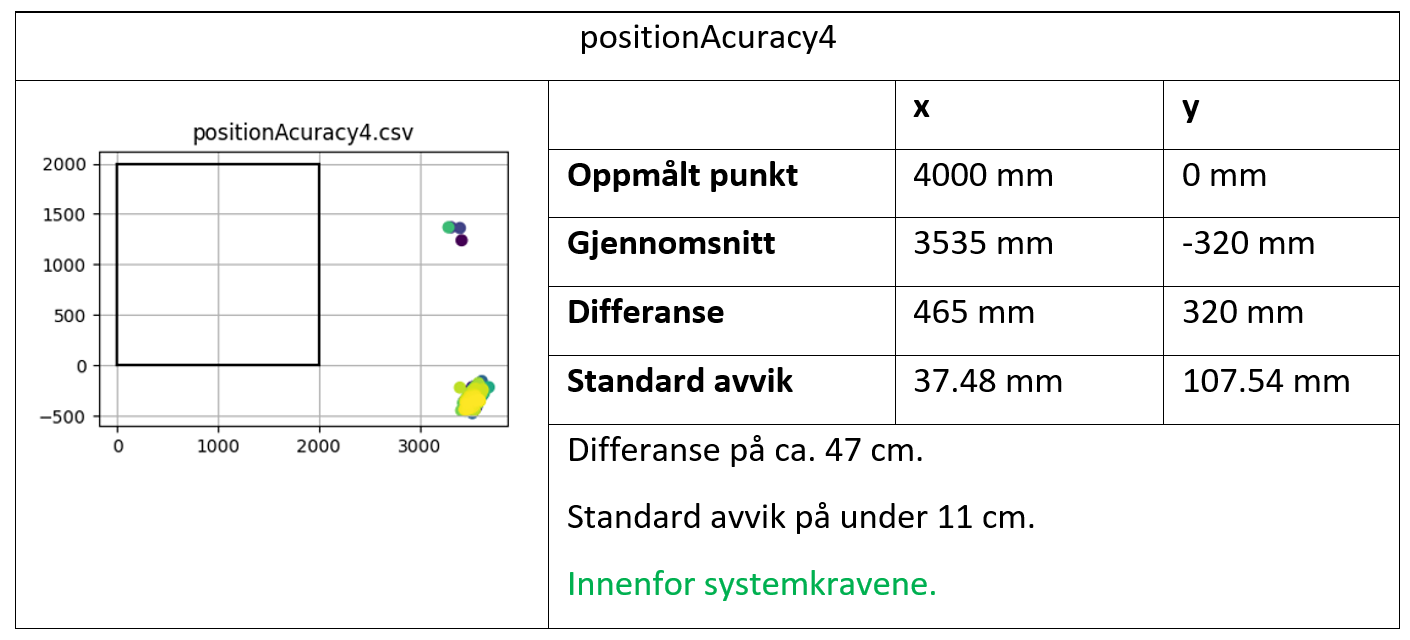
\includegraphics[width=0.5\columnwidth]{figures/2x2resultat4}
\caption{Resultater fra måling 4.}
\label{fig:2x2res4}
\end{figure}

Figur \ref{fig:5x5målinger} og figur \ref{fig:5x5målinger50} viser plot fra logg 6, 7 og 8. 
I figur \ref{fig:5x5målinger50} er de 50 første målingene fjernet for å få bort initialiserings feilmålingene. 

\begin{figure}[htp]
\centering
\includegraphics[width=0.5\columnwidth]{figures/målinger-5x5}
\caption{Målinger med $5\cdot5 m$ ankere.}
\label{fig:5x5målinger}
\end{figure}
\begin{figure}[htp]
\centering
\includegraphics[width=0.5\columnwidth]{figures/målinger-5x5-minus50}
\caption{Målinger med $5\cdot5 m$ ankere uten de 50 første målepunkter.}
\label{fig:5x5målinger50}
\end{figure}

Figur \ref{fig:5x5res6}, {fig:5x5res7} og {fig:5x5res8} under viser de ulike målingene ved 5x5 meter anker oppsett, 
med plot og analyse data.

\begin{figure}[htp]
\centering
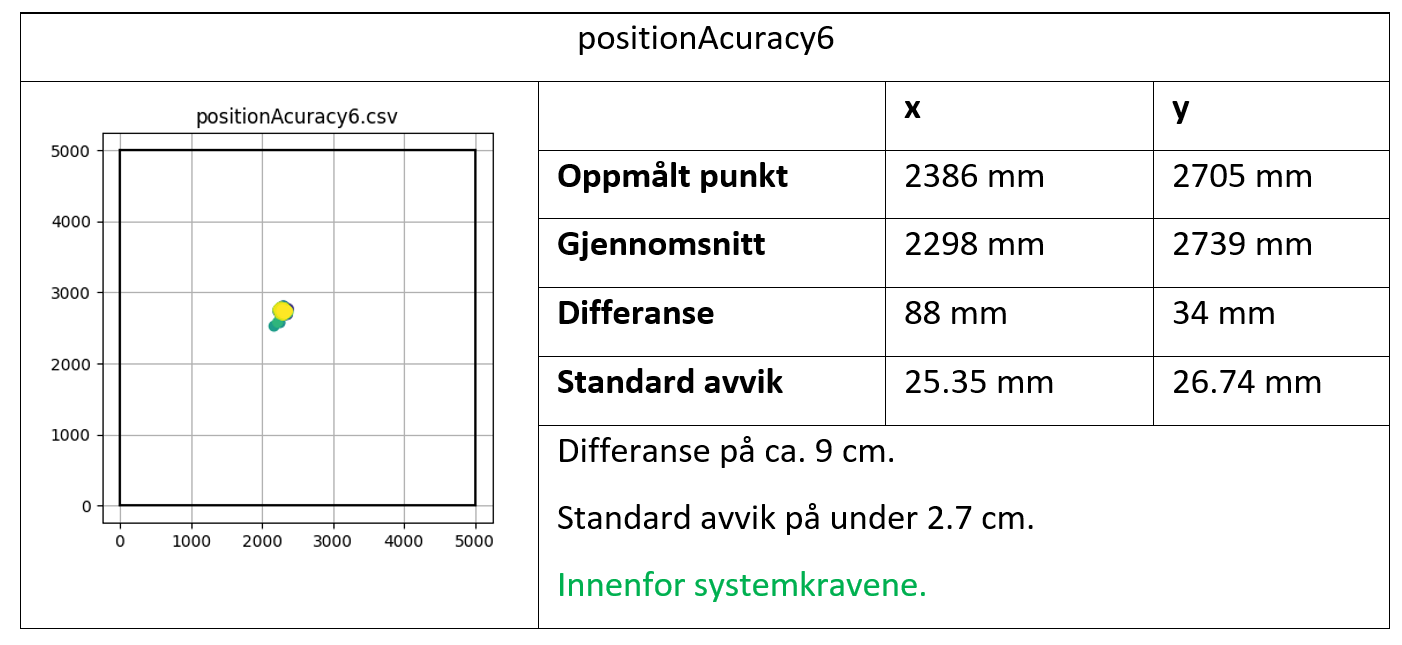
\includegraphics[width=0.5\columnwidth]{figures/5x5-resultat6}
\caption{Resultater fra måling 6.}
\label{fig:5x5res6}
\end{figure}
\begin{figure}[htp]
\centering
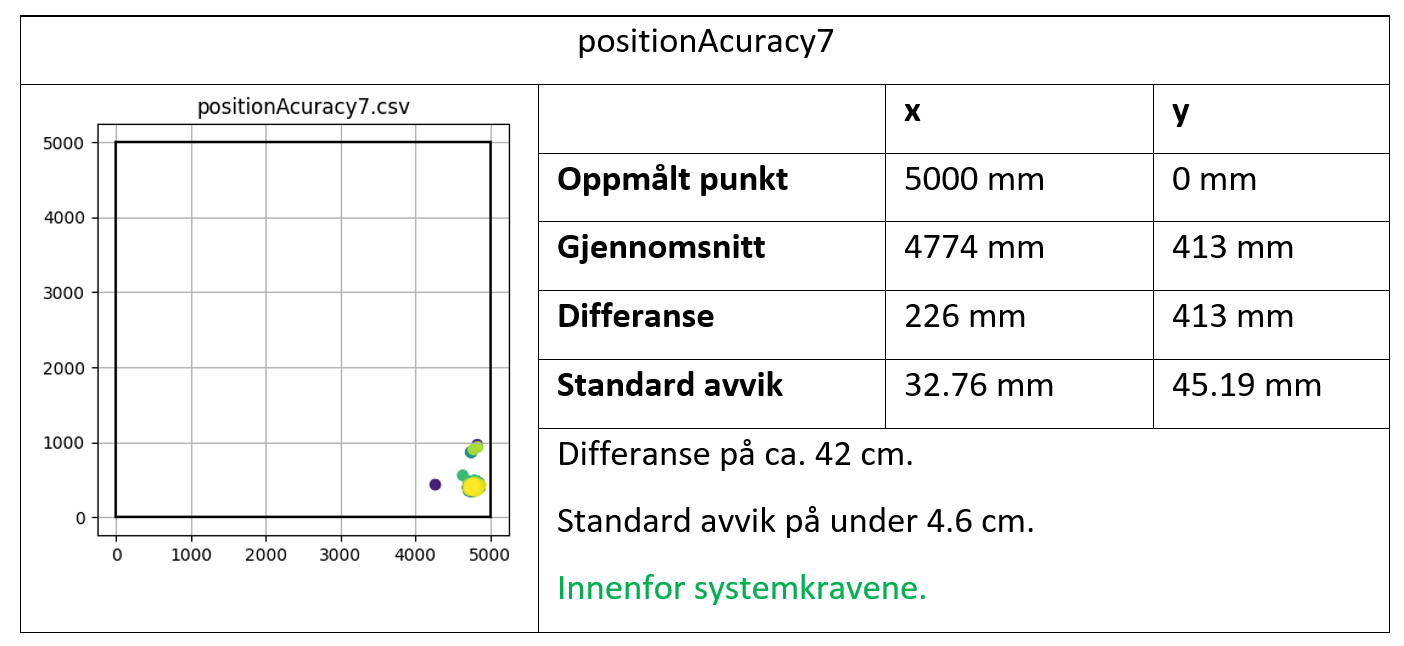
\includegraphics[width=0.5\columnwidth]{figures/5x5-resultat7}
\caption{Resultater fra måling 7.}
\label{fig:5x5res3}
\end{figure}
\begin{figure}[htp]
\centering
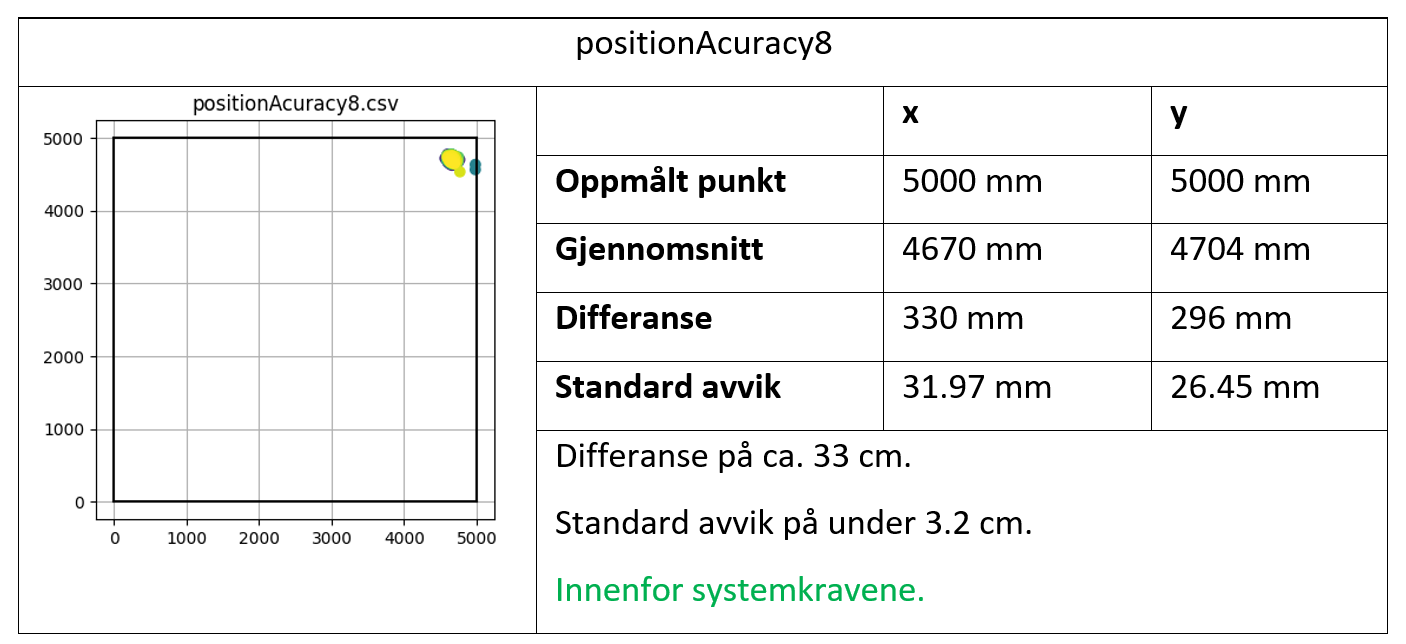
\includegraphics[width=0.5\columnwidth]{figures/5x5-resultat8}
\caption{Resultater fra måling 8.}
\label{fig:5x5res4}
\end{figure}

\newpage
\subsection{Analyse og konklusjon}
Som tabellene for både 2x2 og 5x5 oppsettet viser er det ikke noe merkbar forskjell 
på presisjonene som blir målt. Nøyaktigheten derimot ser ut til å være bedre ved 5x5 oppsettet. 
Der er det største standardavviket på 4.6 cm, mens det for 2x2 er oppe i 11 cm. 
Oppmålingen av anker koordinatene som ble brukt til å regne ut posisjonene er en stor feilkilde i disse testene. 
Bakken der testene ble gjennomført var ikke helt rett, og det var vanskelig å måle nøyaktig med lasermåler på grunn av det sterke sollyset.
Ved å fjerne de 50 første målingene fra testene ble resultantene mye bedre. 
Likevel viser plot 3 og 4 i figur \ref{fig:2x2målinger50} at enda flere målinger burde ha vært fjernet. 
Når systemet brukes for posisjonhold på en drone vil man aldri ta av i løpet av de første sekundene, 
så avviket i initieringsmålingene vil ikke ha noe å si for videre bruk.
Målingene som ble gjort viser at systemet er innenfor kravet om 1m presisjon, og vil derfor kunne brukes videre i prosjektet. 

\subsection{Avlesning av posisjon og oppsett av drone}
Dette kapittelet tar for seg hvordan dronen får posisjon ved hjelp av UWB systemet.
En Pozyx tag, Arduino nano og flightcontroller ble koblet sammen og montert på dronen. 
Pozyx tagen måler avstanden mellom seg og ankerene, og sender disse til Arduinoen. Arduinoen laser av disse avstandene, 
og lager MavLink melinger som vist i figur \ref{fig:melding} slik at Ardupilot kan bruke dataen videre. 
Flightcontrolleren mottar MavLink meldingene, og regner ut posisjonen utafra avstandene til de ulike ankerene. 
Denne kommunikasjonen er illustrert i figur \ref{fig:kommunikasjon}.

\begin{figure}[htp]
\centering
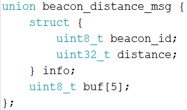
\includegraphics[width=0.5\columnwidth]{figures/melding}
\caption{MavLink melding for anker distanse.}
\label{fig:melding}
\end{figure}

Oppsett av drone:
Det ble utført flere tester av flyvedyktigheten til dronen, etter å fått dronen til å fly var det forbedrigspotensiale i reguleringen. 
Drone fikk osilasjoner som burder bli fikset, men dette måtte bli utført i større lokaler eller utendør når været er bra. 

\begin{figure}[htp]
\centering
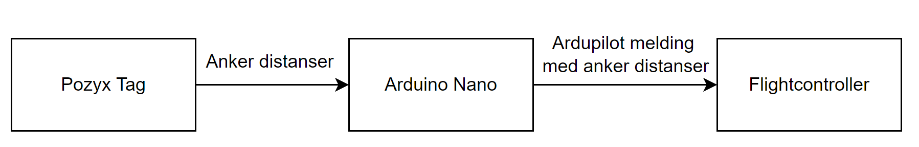
\includegraphics[width=0.5\columnwidth]{figures/kommunikasjon}
\caption{Kommunikasjons vei for tag, arduino og flightcontroller.}
\label{fig:kommunikasjon}
\end{figure}

\subsection{Test av posisjonshold i gang}
Etter å ha fått posisjon estimat i dronen under flyvning, var det neste steget å få dronen til å holde posisjon i luften. 

\subsection{Test av presisjon i krafthallen}
For å få mindre magnetisk forstyrrelse og kunne tune drone bedre, ble det planlagt å fly i krafthallen. 
Autotune, for liten flytid. 

\subsection{Test av posisjonhold I Hamnahallen}
Pid-regulering. 
Loiter test

\subsection{Test av automatisk landing og preprogrammert rute}
Fra tidligere tester hadde dronen suksessfullt klart å holde posisjonen i luften. 
Dronen fløy godt med nye PID-verdier. Vider i planen stod det å teste automatisk landing og flyging med preprogrammert rute. 
Testene ble utført i den eldre gymsalen på kraftsportsenter. 
Der var ankerene satt opp som hamnahallen med 12x12m oppsett i 150cm høyde. 
Før testing ble utført ble oppsettet testet etter sjekklisten. 
Når dronen var koblet opp mot basestasjonen ble dronen bevegd rundt i rommet for å se om posisjonen endret seg riktig. 
En testflight i posisjonhold ble utført for å se om det var noen problem med drone eller posisjonsystemet.  

\subsubsection{Landing}
Dronen ble satt til å lande på en landingspad for å kunne gi indikasjon på treffsikkerheten til systemet. Landingspadden har en diameter på 100cm. 
